\documentclass[12pt]{article}

\usepackage[hidelinks]{hyperref}
\usepackage{graphicx}
\usepackage{color}
\usepackage{xcolor}
\usepackage{listings}
\usepackage{courier}
\usepackage{amsmath}

% syntax highlighting from: http://www.kv0.org/blog/2010/12/15/vernunftiges-syntax-highlighting-in-latex/
\lstset{
	basicstyle=\footnotesize\ttfamily, % Standardschrift
	numbers=left, % Ort der Zeilennummern
	numberstyle=\tiny, % Stil der Zeilennummern
	%stepnumber=2, % Abstand zwischen den Zeilennummern
	numbersep=5pt, % Abstand der Nummern zum Text
	tabsize=2, % Groesse von Tabs
	extendedchars=true, %
	breaklines=true, % Zeilen werden Umgebrochen
	keywordstyle=\color{orange}\bfseries,
	frame=b,
	% keywordstyle=[1]\textbf, % Stil der Keywords
	% keywordstyle=[2]\textbf, %
	% keywordstyle=[3]\textbf, %
	% keywordstyle=[4]\textbf, \sqrt{\sqrt{}} %
	stringstyle=\color{white}\ttfamily, % Farbe der String
	showspaces=false, % Leerzeichen anzeigen ?
	showtabs=false, % Tabs anzeigen ?
	xleftmargin=17pt,
	framexleftmargin=17pt,
	framexrightmargin=5pt,
	framexbottommargin=4pt,
	commentstyle=\color{green},
	% backgroundcolor=\color{gray},
	showstringspaces=false, % Leerzeichen in Strings anzeigen ?
	morekeywords={__global__} % CUDA specific keywords
}
\lstloadlanguages{% Check Dokumentation for further languages ...
%[Visual]Basic
%Pascal
C,
C++,
%XML
%HTML
Java
}
%\DeclareCaptionFont{blue}{\color{blue}}
 
%\captionsetup[lstlisting]{singlelinecheck=false, labelfont={blue}, textfont={blue}}
\usepackage{caption}
\DeclareCaptionFont{white}{\color{white}}
\DeclareCaptionFormat{listing}{\colorbox{gray}{\parbox{\textwidth}{\hspace{15pt}#1#2#3}}}
\captionsetup[lstlisting]{format=listing,labelfont=white,textfont=white, singlelinecheck=false, margin=0pt, font={bf,footnotesize}}

\title{Project Report - Third assignment - GAME ENGINES}
\author{Andrea Distler}
\date{10 December, 2012}

\begin{document}
\maketitle
\newpage

\tableofcontents
\newpage

%------------------------------------------
\section{Introduction}
This is the project report for the third assignment of the Game Engines course.

A short description of the source code and the used libraries can be found in section \ref{section:files}. The files are available on GitHub.

In section \ref{section:outcome} the outcome is described. In section \ref{section:classes} used mechanics and an overview of the classes can be found.

%------------------------------------------
\section{The Files}
\label{section:files}
All files can be found on GitHub. \newline 
\url{https://github.com/JungleJinn/GE---SimplePlatformerEngine}.

The project was written in C++, without using additional libraries.

%------------------------------------------
\section{Outcome}
\label{section:outcome}

The assignment was to implement the A* search algorithm on a grid-formed graph. There should be two ``NPCs'', which navigate using a finite state machine. In my project, the NPCs have each two states: a chase state and a flee state. The NPC in the chase state is represented by an upper-case letter, the NPC in the flee state is depicted as a lower-case letter. An ``X'' marks which grid nodes are blocked. Figure \ref{figure:outcome} shows the output of the application.

\begin{figure}[H]
	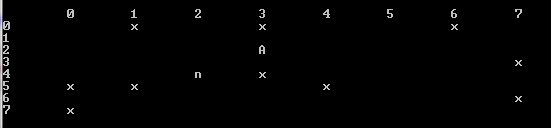
\includegraphics[width=\textwidth]{screenshot.png}
	\caption{A screenshot of the result.}
	\label{figure:outcome}
\end{figure}

% -----------------------------------------
\section{Classes and Mechanics}
\label{section:classes}


\paragraph{Graph and Node.}
The Graph and Node classes are the basic classes used to form the structure of the grid and the gridnodes. They are also tools to visualize that the grid is handled like a graph.

\paragraph{Link.}
The Link class links two nodes of an arbitrary type. It can also store an edge travel cost.

\paragraph{Grid.}
The Grid class basically manages everything. It derives from the Graph class and contains a list of all its nodes. It also contains the two NPCs. It naturally handles the creation of the nodes and their links.

\paragraph{GridNode.}
The GridNodes play an essential role in the calculation of paths. They store their temporary costs and heuristic costs. This means that there could not be two A* path-finding algorithms running at the same time.

\paragraph{FiniteStateMachine(FSM).}

In listing \ref{listing:fsm} the finite state machine is shown. It holds the current state and handles state changes by calling the enter and exit methods of the states.

\begin{lstlisting}[caption=The finite state machine.,label=listing:fsm,language=C++]
template <typename T>
public class FSM
{
public:

							FSM(FSMState<T> *state)
							{
								lastState = NULL;
								currentState = state;
							}

	void					ChangeState(FSMState<T> *newState)
	{
		if (currentState != newState)
		{
			lastState = currentState;

			lastState->Exit();
			
			currentState = newState;
			currentState->Enter();
		}
	}

protected:
	FSMState<T> *			lastState;
	FSMState<T> *			currentState;
};
\end{lstlisting}

\paragraph{FSMState.}

The FSM contains only states of a certain pattern, like in listing \ref{listing:fsmstate}. Both the ChaseState and the FleeState derive from this class.

\begin{lstlisting}[caption=A finite state machine state.,label=listing:fsmstate,language=C++]
template <typename T>
public class FSMState
{
public:
							FSMState(T *_owner)
							{
								owner = _owner;
							}

	virtual void			Enter() = 0;
	virtual void			Update(/*float deltaTime*/) = 0;
	virtual void			Exit() = 0;

	//char*					Name;

protected:
	T*						owner;
};
\end{lstlisting}

\paragraph{NPC.}
The NPC class derives from the FSM, as shown in listing \ref{listing:npc}. It stores instances of the states it needs. The best next node to move to is calculated in the ChaseState. The FleeState doesn't do much more than randomly choosing new nodes after five turns.

\begin{lstlisting}[caption=Curiously recurring template pattern., label=listing:npc,language=C++]
class NPC : public FSM<NPC>
{
public:

	ChaseState*				chaseState;
	FleeState*				fleeState;
	
	.
	.
	.
};
\end{lstlisting}

\lstlistoflistings
\listoffigures

\end{document}